\documentclass[../main.tex]{subfiles}

\begin{document}

The model was trained on a NVIDIA RTX A500 laptop GPU, in batches of 5 images. The model was left to train for 2 days (50 epochs). The resulting loss and accuracy graphs can be seen on figures \ref{fig:training:loss} and \ref{fig:training:accuracy}.

\begin{figure}[htb]
    \centering

    \begin{tikzpicture}
        \begin{axis}[
                xlabel = epoch,
                ylabel = loss,
                xmin=0, xmax=50,
                width=.9\textwidth,
                height=.4\textwidth,
                legend style = {at={(1, 1)}, anchor=south east}
            ]

            \addplot[
                color = red,
                mark = o,
                mark size = 1.5pt
            ]
            table[x=epoch, y=training_loss]{training/training.csv};
            \addlegendentry{Training loss}

            \addplot[
                color = blue,
                mark = square,
                mark size = 1.5pt,
            ]
            table[x=epoch, y=validation_loss]{training/training.csv};
            \addlegendentry{Validation loss}

        \end{axis}
    \end{tikzpicture}

    \caption{Loss graph (training \& accuracy)}
    \label{fig:training:loss}

\end{figure}

\begin{figure}[htb]
    \centering 

    \begin{tikzpicture}
        \begin{axis}[
                xlabel = epoch,
                ylabel = accuracy (\%),
                xmin=0, xmax=50,
                width=.9\textwidth,
                height=.4\textwidth
            ]

            \addplot[
                mark = square,
                mark size = 1.5pt
            ]
            table[x=epoch, y=validation_accuracy]{training/training.csv};

        \end{axis}
    \end{tikzpicture}

    \caption{Validation accuracy graph}
    \label{fig:training:accuracy}
\end{figure}

Looking at the loss graph, whilst a decreasing trend can be seen for training loss, no obvious trend is present in validation loss data. Validation accuracy also shows no progress over epochs 0-50.

An example image from the dataset was passed to the model to see how well it performs. Input, truth mask and the predicted mask images can be seen on figure \ref{fig:training:image}

\begin{figure}
\centering

\begin{subfigure}{.3\textwidth}
    \centering
    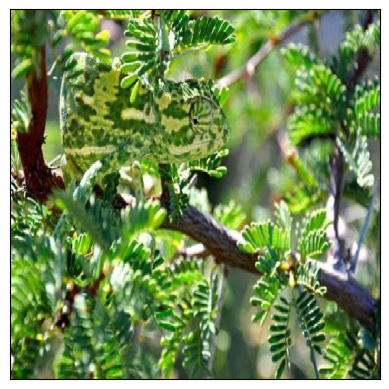
\includegraphics[width=\textwidth]{training/input.png}
    \caption{Input}
\end{subfigure}
\begin{subfigure}{.3\textwidth}
    \centering
    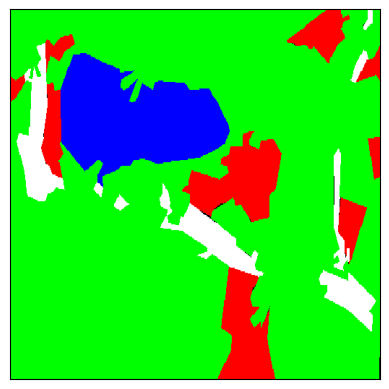
\includegraphics[width=\textwidth]{training/truth.png}
    \caption{Truth}
\end{subfigure}
\begin{subfigure}{.3\textwidth}
    \centering
    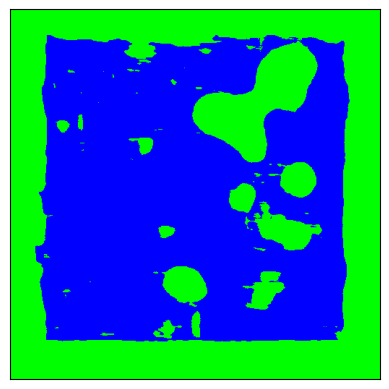
\includegraphics[width=\textwidth]{training/prediction.png}
    \caption{Prediction}
\end{subfigure}

\caption{Input, truth mask and predicted mask after 50 epochs of training}
\label{fig:training:image}

\end{figure}

As can be seen, the model failed to achieve it task of finding camouflaged animals on an image. The resulting prediction preserves no hint of the original image, and shows that the model has a preference to assigning pixels to the camouflaged animal group.

\end{document}